\subsection{@title@}
\begin{figure}[H]
  \center\includegraphics[width=0.6\textwidth]{@fig_param@.param/calc_likelihood_bounds.py/fig1.png}
  \caption{Likelihood on a parameter grid around the best mode. The marginalized parameter likelihood have
    1 $\sigma$ areas shaded in blue. The 2D likelihood distributions have 1 $\sigma$  and 2 $\sigma$ contours}
  \label{fig:basic_rd:likelihood}
\end{figure}

\begin{figure}[H]
  \center\includegraphics[width=0.6\textwidth]{@fig_param@.param/calc_likelihood_bounds.py/fig2.png}
  \caption{Likelihood on a parameter grid around the best mode. The marginalized parameter likelihood have
    1 $\sigma$ areas shaded in blue. The 2D likelihood distributions have 1 $\sigma$  and 2 $\sigma$ contours}
  \label{fig:basic_rd:likelihood}
\end{figure}

\begin{figure}[H]
  \center\includegraphics[width=0.6\textwidth]{@fig_param@_zoom.param/calc_likelihood_bounds.py/fig1.png}
  \caption{Likelihood on a parameter grid around the best mode. The marginalized parameter likelihood have
    1 $\sigma$ areas shaded in blue. The 2D likelihood distributions have 1 $\sigma$  and 2 $\sigma$ contours}
  \label{fig:basic_rd:likelihood}
\end{figure}

\begin{figure}[H]
  \center\includegraphics[width=0.6\textwidth]{@fig_param@_zoom.param/calc_likelihood_bounds.py/fig2.png}
  \caption{Likelihood on a parameter grid around the best mode. The marginalized parameter likelihood have
    1 $\sigma$ areas shaded in blue. The 2D likelihood distributions have 1 $\sigma$  and 2 $\sigma$ contours}
  \label{fig:basic_rd:likelihood}
\end{figure}


\begin{figure}
  \begin{subfigure}{.5\textwidth}
    \centering\includegraphics[width=1.0\linewidth]{@fig_param@.param/plot_zmrs.py/fig2.png}
    \caption{a}
  \end{subfigure}
  \begin{subfigure}{.5\textwidth}
    \centering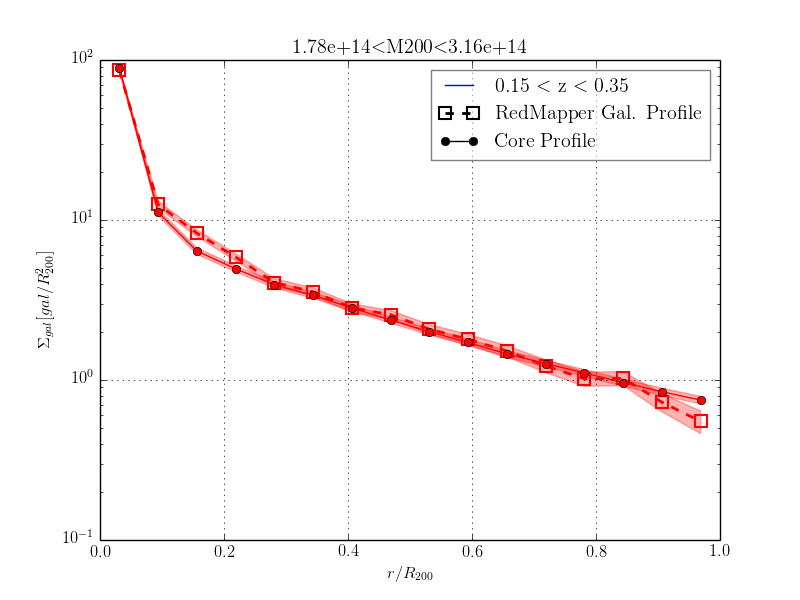
\includegraphics[width=1.0\linewidth]{@fig_param@.param/plot_zmrs.py/fig3.png}
    \caption{a}
  \end{subfigure}
  \begin{subfigure}{.5\textwidth}
    \centering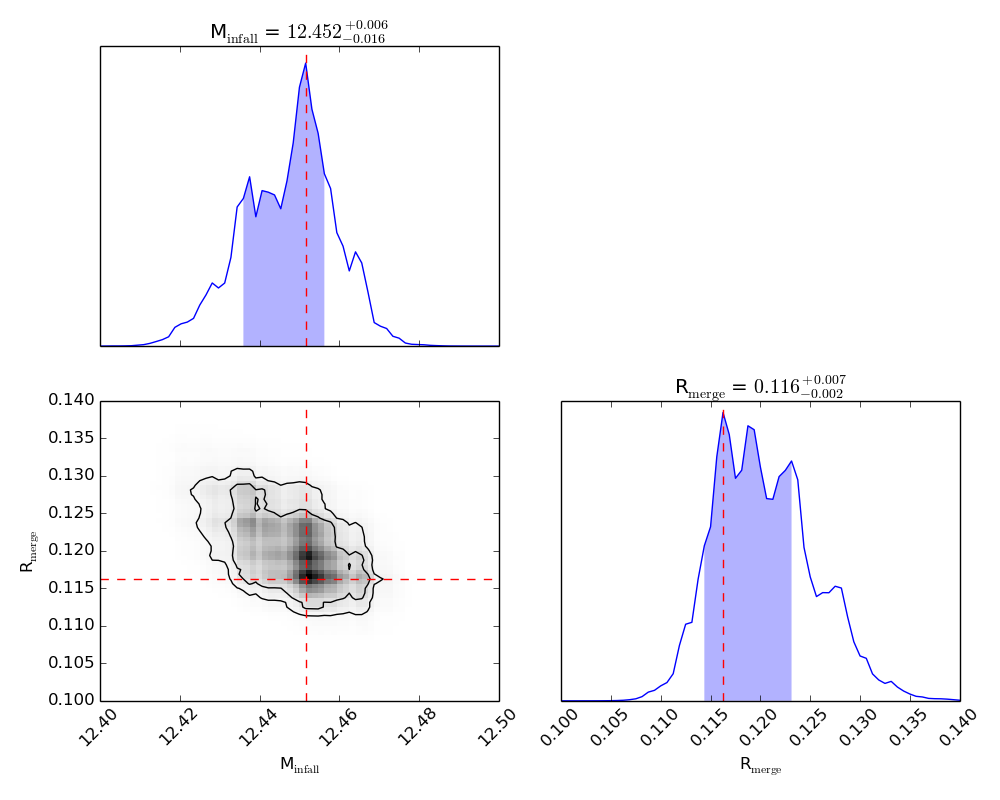
\includegraphics[width=1.0\linewidth]{@fig_param@.param/plot_zmrs.py/fig4.png}
    \caption{a}
  \end{subfigure}%
  \begin{subfigure}{.5\textwidth}
    \centering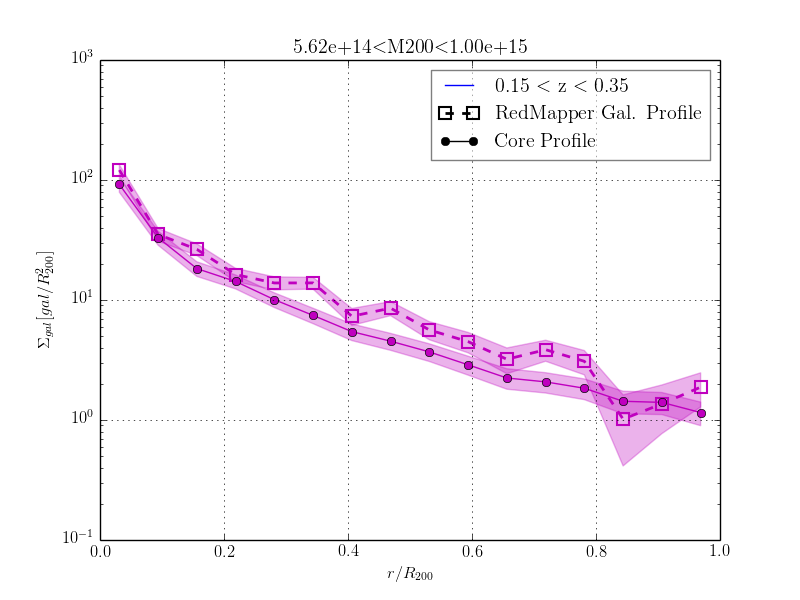
\includegraphics[width=1.0\linewidth]{@fig_param@.param/plot_zmrs.py/fig5.png}
    \caption{a}
  \end{subfigure}
  \begin{subfigure}{.5\textwidth}
    \centering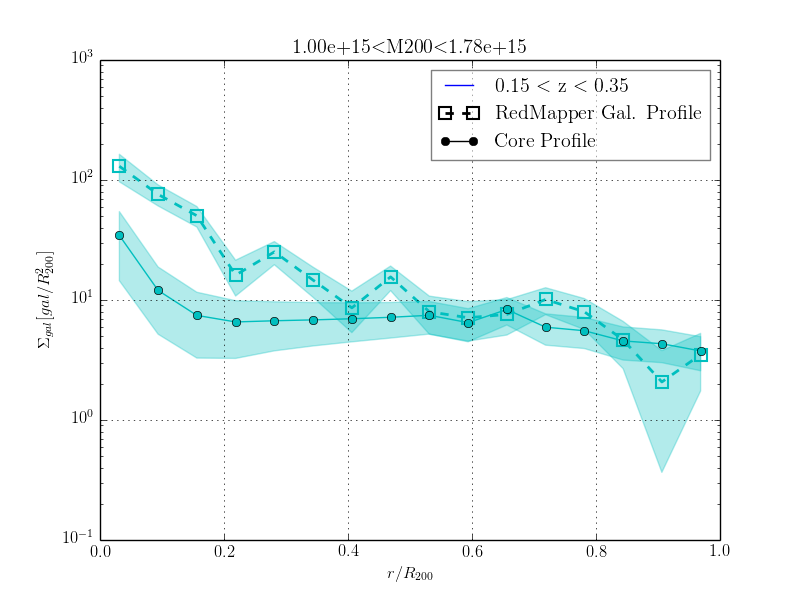
\includegraphics[width=1.0\linewidth]{@fig_param@.param/plot_zmrs.py/fig6.png}
    \caption{a}
  \end{subfigure}
  
\end{figure}
\clearpage
